\documentclass[a4paper, 11pt]{article}
\usepackage{geometry}
\geometry{letterpaper, margin=1in}
\usepackage{graphicx}
\graphicspath{ {images/} }

\usepackage{amsmath}
\usepackage{amssymb}  
\usepackage{amsthm}
\usepackage{ulem}

\usepackage{enumitem}


\usepackage{pdfpages} % for including full pdf pages

\usepackage{empheq}

\usepackage{listings}


%format to allow bolded theorems, corollaries, etc...
\newtheorem*{theorem}{Theorem}
\newtheorem*{corollary}{Corollary}
\newtheorem*{lemma}{Lemma}
\newtheorem*{definition}{Definition}
\newtheorem*{Example}{Example} 
\newtheorem*{Remark}{Remark}

% stop typing \mathbb a thousand times 
\newcommand{\R}{\mathbb{R}}
\newcommand{\C}{\mathbb{C}}
\newcommand{\F}{\mathbb{F}}
\newcommand{\E}{\mathbb{E}}
\newcommand{\M}{\mathbb{M}}
\newcommand{\sphere}{\mathbb{S}}

% commands for bra-ket notation
\newcommand{\bra}[1]{\ensuremath{\left\langle#1\right|}}
\newcommand{\ket}[1]{\ensuremath{\left|#1\right\rangle}}
\newcommand{\bracket}[2]{\ensuremath{\left\langle #1 \middle| #2 \right\rangle}}
\newcommand{\matrixel}[3]{\ensuremath{\left\langle #1 \middle| #2 \middle| #3 \right\rangle}}
\newcommand{\expectation}[1]{\ensuremath{\left\langle #1 \right\rangle}}

% vector stuff
\newcommand{\basis}[1]{\hat{\mathbf{e}}_#1}
\newcommand{\unit}[1]{\hat{\boldsymbol{#1}}}
\newcommand{\bvec}[1]{\vec{\boldsymbol{#1}}}
\newcommand{\threevec}[2]{\begin{pmatrix} #1 \\ #2 \end{pmatrix}}

% change margins for solution
\newenvironment{solution}{%
	\begin{list}{}{%
			\setlength{\topsep}{0pt}%
			\setlength{\leftmargin}{0.5cm}%
			\setlength{\rightmargin}{0.5cm}%
			\setlength{\listparindent}{\parindent}%
			\setlength{\itemindent}{\parindent}%
			\setlength{\parsep}{\parskip}%
		}%
		\item[]}{\end{list}}




\begin{document}
\noindent
\large\textbf{Homework 1} \hfill \textbf{John Waczak} \\
\normalsize PH 653 \hfill  Date: \today \\
Dr. Oksana Ostroverkhova \hfill worked w/ Ryan Tollefsen
\par\noindent\rule{\textwidth}{0.4pt} \\\\



\begin{enumerate}[leftmargin=0em, label=\textbf{\arabic*}]
  \item Consider hydrogen atom. Apply the variational method and calculate an
approximate value for the energy of the ground state using the following trial
functions:
  \begin{align*}
    &(a)\qquad \psi_a = e^{-ar}, \qquad a>0\\
    &(b)\qquad \psi_a = re^{-ar}, \qquad a>0\\
    &(c)\qquad \psi_a = \frac{r}{r^2+a^2} \\
    &(d)\qquad \psi_a = \frac{1}{r^2+a^2}
  \end{align*}
  In each case, compare the approximate result to the energy values obtained via exact
calculation. Which trial function yields the energy value which agrees the best with the
exact value?

  \begin{solution}
      To estimate the energy of the ground state, we must minimize the
      expectation value of the Hamiltonian with respect to the parameter a for
      a test function $\psi_a$, i.e.
      \begin{equation}
        \expectation{\hat{H}}(a) = \frac{\matrixel{\psi_a}{\hat{H}}{\psi_a}}{\bracket{\psi_a}{\psi_a}}
      \end{equation}

      It is best if we start with the normalization factor
      $\bracket{\psi_a}{\psi_a}$ as this will allow us to check if $\psi_a$ is
      reasonable before continuing with the harder
      $\matrixel{\psi_a}{\hat{H}}{\psi_a}$ calculation.
      \begin{align}
        \bracket{\psi_a}{\psi_a} &= \int_0^\infty\int_0^\pi\int_0^{2\pi}r^2\sin\theta\;drd\theta d\phi \left| \psi_a(r) \right|^2\\
      \end{align}

      Recalling the useful integral identity
      \begin{equation}
        \int_0^\infty x^n e^{-\alpha x}dx = \frac{\Gamma(n+1)}{\alpha^{n+1}}
      \end{equation}
      enables us to solve the integrals.\\
      
      Having chosen a reasonably behaved test function we may continue with the
      calculation. We now must calculate the matrix element
      $\matrixel{\psi_a}{\hat{H}}{\psi_a}$. For the hydrogen atom, our Hamiltonian is
      given by
      
      \begin{align}
        \hat{H} &= -\frac{\hbar^2}{2\mu}\nabla^2-\frac{1}{4\pi\epsilon_0}\frac{q^2}{r} \\
        &= -\frac{\hbar^2}{2\mu}\frac{1}{r^2}\frac{\partial}{\partial r}\left( r^2\frac{\partial}{\partial r} \right) - \frac{1}{4\pi\epsilon_0}\frac{q^2}{r}
      \end{align}
      where the final line follows as $\psi_a$ only has $r$ dependence. With
      this, the matrix element becomes
      \begin{align}
        \matrixel{\psi_a}{\hat{H}}{\psi_a} &= 4\pi \int_0^\infty \psi_a\Big[\hat{H}\; \psi_a \Big]r^2dr 
      \end{align}

      To save time, I've calculated the value of these two integrals for each
      test function in the following Mathematica notebook.
      
      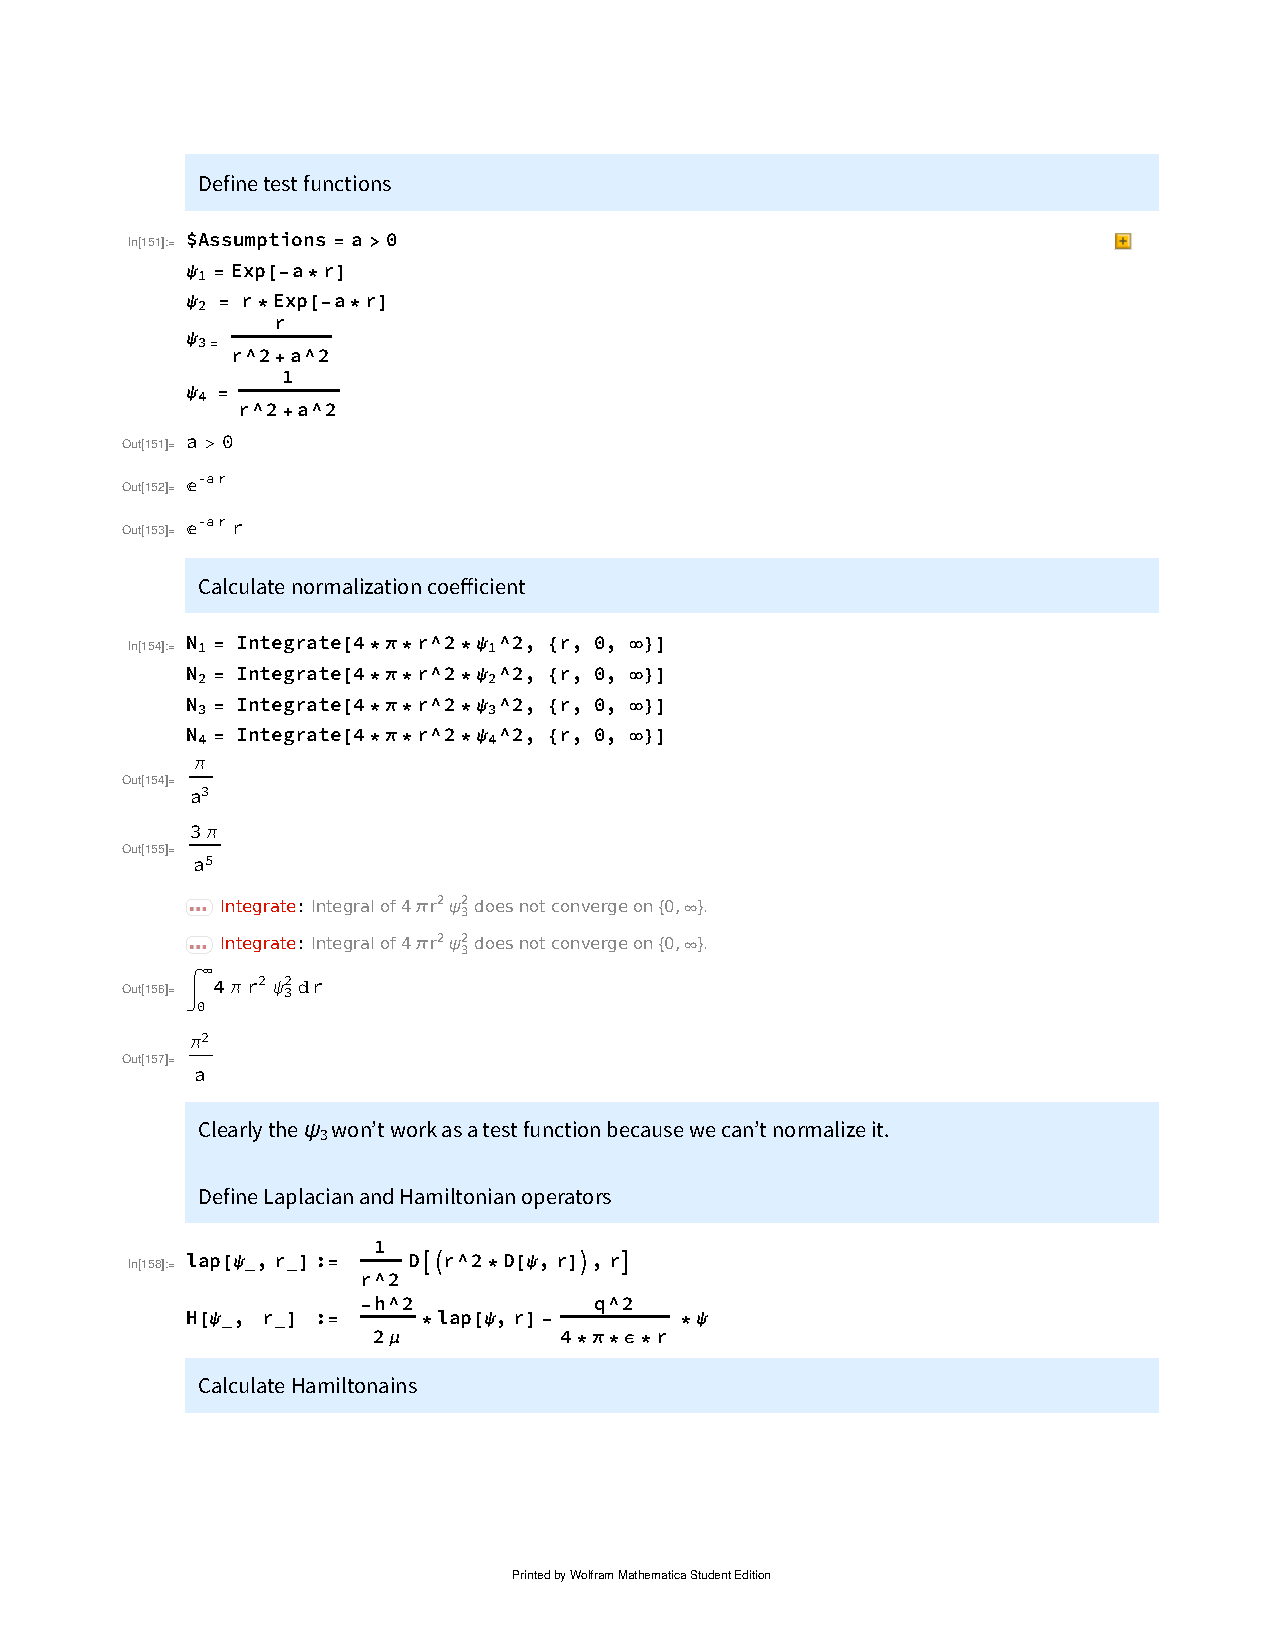
\includepdf[pages=-]{notebook.pdf}

      In summary we found that $\psi_a=\frac{r}{r^2+a^2}$ is not a suitable test
      function and that for the other three functions, the parametrized
      expectation value is
      \begin{align}
        &(a)\qquad \hat{\expectation{H}}(a) = \frac{a^2h^2}{2\mu}-\frac{aq^2}{4\pi\epsilon_0}\\
        &(b)\qquad \hat{\expectation{H}}(a) = \frac{a^2\hbar^2}{6\mu}-\frac{aq^2}{8\pi\epsilon_0}\\
        &(d)\qquad \hat{\expectation{H}}(a) = \frac{\hbar^2}{4a^2\mu}-\frac{q^2}{2a\pi^2\epsilon_0}
      \end{align}
      Now we can take the derivative of these equations w.r.t. $a$ in order to
      minimize for the ground state energy estimate.
      \begin{align}
        &(a)\qquad \frac{\partial}{\partial a}\hat{\expectation{H}}(a) =  \frac{a\hbar^2}{\mu} - \frac{q^2}{4\pi\epsilon_0}\\ 
        &(b)\qquad \frac{\partial}{\partial a}\hat{\expectation{H}}(a) = \frac{a\hbar^2}{3\mu}-\frac{q^2}{8\pi\epsilon_0}\\
        &(d)\qquad \frac{\partial}{\partial a}\hat{\expectation{H}}(a) = -\frac{\hbar^2}{2a^3\mu}+\frac{q^2}{2a^2\pi^2\epsilon_0}
      \end{align}
      Setting each of these equations equal to zero and solving for $a$ yields
      \begin{align}
        &(a)\qquad a = \frac{q^2\mu}{4\hbar^2\pi\epsilon_0}\\
        &(b)\qquad a = \frac{3q^2\mu}{8\hbar^2\pi\epsilon_0}\\
        &(d)\qquad a = \frac{\hbar^2\pi^2\epsilon_0}{q^2\mu}
      \end{align}
      Finally, re-substituting into previous set of equations gives the ground
      state energy estimates for each test function.
       \begin{align}
        &(a)\qquad E_{gs} \approx -\frac{q^4\mu}{32\hbar^2\pi^2\epsilon_0^2}\\
        &(b)\qquad E_{gs} \approx -\frac{3q^4\mu}{128\hbar^2\pi^2\varepsilon_0^2}\\
        &(d)\qquad E_{gs} \approx -\frac{q^4\mu}{4\hbar^2\pi^4\epsilon_0^2}
      \end{align}
 
    \end{solution}







  
  \item Consider a 1D system only having, i.e.
    $H_0\ket{\varphi_n}=E_n\ket{\varphi_n}$, $n=1,2$. At $t=0$, a perturbation
    $V(x,t)=V(x)$ is turned on, where $V$ is a real function. It is also known
    that this perturbation has no diagonal elements when represented in
    $\{\ket{\varphi_n}\}$ basis, i.e. $\matrixel{\varphi_i}{V}{\varphi_i}=0$. At
    $t=0$, the populations of the states 1 and 2 was $P_1(0)=1$ and $P_2(0)=0$,
    respectively. Find the populations of the two states as a function of time
    and of the matrix elements $\matrixel{\varphi_1}{V}{\varphi_2} = V_{12}$ for
    the special case that the states are degenerate, i.e. $E_1 = E_2$. Sketch
    $P_1$ and $P_2$ as functions of time.  \\

    \begin{solution}
      Given that $H_0\ket{\varphi_n}=E_n\ket{\varphi_n}$ and that
      $V(x,t)=V(x)$ for $t>0$, recall that the interaction picture
      ``Schrodinger'' equation becomes
      \begin{equation}
        i\hbar\frac{d}{d t}c_n(t) = \sum_m V_{nm}e^{i\omega_{nm}t}c_m(t)
      \end{equation}
      where
      \begin{equation}
        \omega_{nm}= (E_n-E_m)/\hbar
      \end{equation}
      Because $E_1=E_2$ it therefore follows that $\omega_{12}=\omega_{21}=0$.
      Furthermore, because there are no diagonal terms in $V$, we have that
      $V_{11}=V_{22}=0$. Thus, the differential equation reduces to a system of
      two coupled ODEs.
      \begin{align}
        i\hbar\;\dot c_1(t) &= V_{12}c_2(t) \\
        i\hbar\;\dot c_2(t) &= V_{21}c_1(t)
      \end{align}
      using the trick from class, we can take a derivative of both equations and
      substitute in order to decouple.
      \begin{align}
        i\hbar \ddot c_1(t) &= \dot V_{12}c_2(t)+V_{12}\dot c_2(t) \\
        i\hbar \ddot c_2(t) &= \dot V_{21}c_1(t)+V_{21}\dot c_1(t) \\
        \dot c_1 &= -\frac{i}{\hbar}V_{12}c_2(t) \\
        \dot c_2 &= -\frac{i}{\hbar}V_{21}c_1(t) \\
        \Rightarrow \ddot c_1 - &\left( \frac{\dot V_{12}}{V_{12}} \right)\dot c_1 + \frac{V_{12}V_{21}}{\hbar^2}c_1 = 0 \\
        \Rightarrow \ddot c_2 - &\left( \frac{\dot V_{21}}{V_{21}} \right)\dot c_2 + \frac{V_{12}V_{21}}{\hbar^2}c_2 = 0 
      \end{align}
      
      We can further simplify the final two equations from above by realizing
      that because $V(x,t)=V(x)$, then $V_{12}=V_{12}(x)$ and $V_{21}=
      V_{21}(x)$ so that $\dot V_{12}=\dot V_{21} = 0$. \\

      \begin{align}
        \ddot c_1 + \frac{V_{12}V_{21}}{\hbar^2}c_1 &= 0 \\
        \ddot c_2 + \frac{V_{12}V_{21}}{\hbar^2}c_2 &= 0 
      \end{align}
      Our boundary conditions then yield $c_1(0)=1$ and $c_2(0)=0$ so that the
      time dependence of populations is given by
      \begin{align}
        c_1(t) &= \cos\left(\frac{V_{12}V_{21}}{\hbar^2}t\right) \\ 
        c_2(t) &= \sin\left(\frac{V_{12}V_{21}}{\hbar^2}t\right) \\ 
        P_1(t) &= \cos^2\left(\frac{V_{12}V_{21}}{\hbar^2}t\right) \\ 
        P_2(t) &= \sin^2\left(\frac{V_{12}V_{21}}{\hbar^2}t\right) 
      \end{align}
      A sketch of the populations is shown below
      \begin{figure}[!hbt]
        \centering
        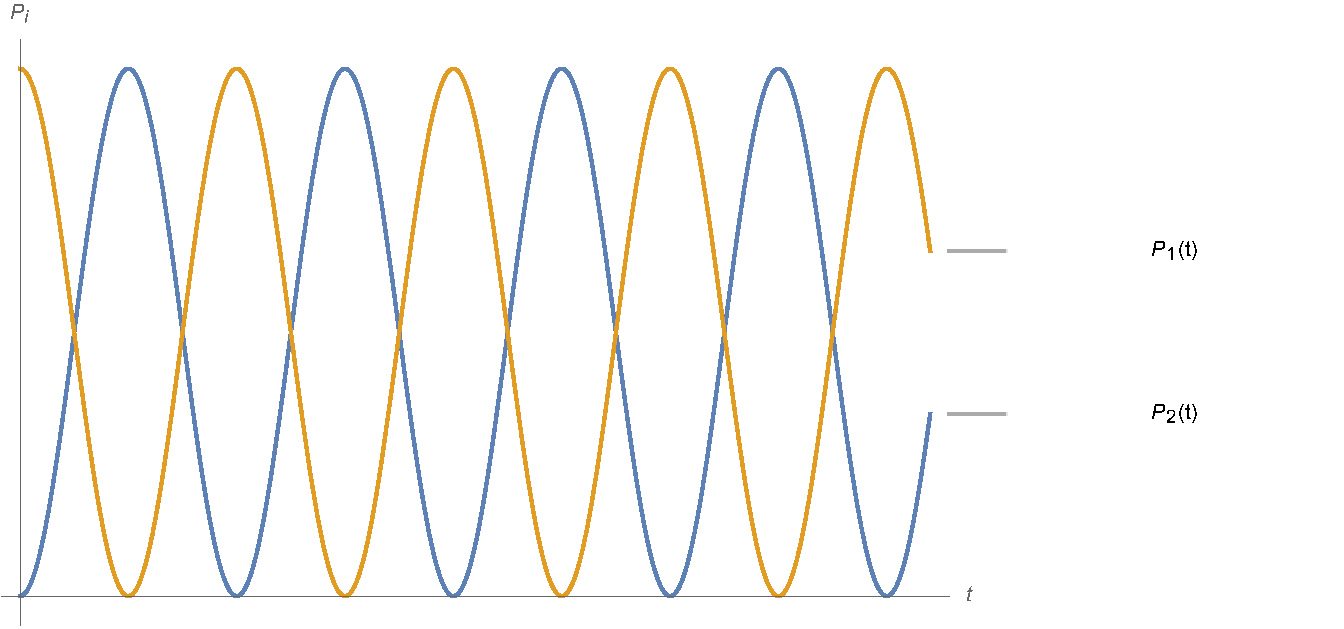
\includegraphics[width=1\columnwidth]{sketch}
        \caption{\textbf{Time dependent populations} figure comparing population
        1 and 2.}
      \end{figure}
      

    \end{solution}
    


\end{enumerate}

  
\end{document}






























